\documentclass[12pt,fleqn]{article}\usepackage{../common}
\begin{document}
Ozet Istatistikleri, Grafikleri

\begin{minted}[fontsize=\footnotesize]{python}
import pandas as pd
df = pd.read_csv('iris.csv')
df = df.ix[:,0:4]
pd.scatter_matrix(df)
plt.savefig('stat_summary_01.png')
\end{minted}

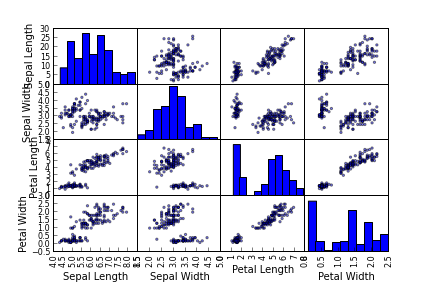
\includegraphics[height=8cm]{stat_summary_01.png}

\begin{minted}[fontsize=\footnotesize]{python}
print df.cov()
\end{minted}

\begin{verbatim}
              Sepal Length  Sepal Width  Petal Length  Petal Width
Sepal Length      0.685694    -0.039268      1.273682     0.516904
Sepal Width      -0.039268     0.188004     -0.321713    -0.117981
Petal Length      1.273682    -0.321713      3.113179     1.296387
Petal Width       0.516904    -0.117981      1.296387     0.582414
\end{verbatim}

\begin{minted}[fontsize=\footnotesize]{python}
means = df.mean()
df2 = df.apply(lambda x: x - means, axis=1)
print np.dot(df2.T,df2) / df.shape[0]
\end{minted}

\begin{verbatim}
[[ 0.68112222 -0.03900667  1.26519111  0.51345778]
 [-0.03900667  0.18675067 -0.319568   -0.11719467]
 [ 1.26519111 -0.319568    3.09242489  1.28774489]
 [ 0.51345778 -0.11719467  1.28774489  0.57853156]]
\end{verbatim}


Ortalama (Mean) ve Medyan (Median)

Genellikle istatistik kitaplari hemen ortalama (mean), medyan (median) ve
baglantili ozet istatistiklerinden (summary statistics) bahsederek ise
girerler. Bu istatistikleri dikkatle kullanmak gerekir, cunku her turlu
veri, her yerde gecerli degildirler. Mesela ortalama sadece tek merkezi bir
tepesi olan (unimodal) dagilimlar icin gecerlidir. Eger bu temel varsayim
gecerli degilse, ortalama kullanarak yapilan hesaplar bizi yanlis yollara
goturur. Ayrica bir dagilimi simetrik olup olmadigi da ortalama ya da
medyan kullanilip kullanilmamasi kararinda onemlidir. Eger simetrik, tek
tepeli bir dagilim var ise, ortalama ve medyan birbirine yakin
olacaktir. Fakat veri baska turde bir dagilim ise, o zaman bu iki olcut
birbirinden cok farkli olabilir.

Once ortalama ve standart sapmayi (standart deviation) gorelim.

$$ m  = \frac{ 1}{n}\sum_i x_i $$

Standart sapma veri noktalarin "ortalamadan farkinin ortalamasini"
verir. Tabii bazen noktalar ortalamanin altinda, bazen ustunde olacaktir,
bizi bu negatiflik, pozitiflik ilgilendirmez, biz sadece farkla
alakaliyiz. O yuzden her sapmanin karesini aliriz, bunlari toplayip nokta
sayisina boleriz .

$$ s^2 = \frac{ 1}{n} \sum_i (x_i - m)^2 $$

Eger $m$ tanimini ustte yerine koyarsak, 

$$ = \frac{ 1}{n} \sum_i x_i^2 + \frac{ 1}{n} \sum_i m^2 - \frac{ 2}{n} \sum_i x_im  $$

$$ = \frac{ 1}{n} \sum_i x_i^2 + \frac{ m^2n}{n} - \frac{ 2mn}{n}m $$

$$ = \frac{ 1}{n} \sum_i x_i^2 +  m^2 - 2m^2 $$

$$ = \frac{ 1}{n} \sum_i x_i^2 - m^2 $$

Bu olcuye varyans (variance) denir ve teorik olarak ortalamadan daha onemli
oldugu soylenebilir. Fakat dagilimin yayilma olcusu olarak biz bu olcuyu
oldugu gibi degil, onun karesini kullanacagiz (ki standart sapma buna
deniyor aslinda). Niye? Cunku o zaman veri noktalarinin ve yayilma olcusunun
birimleri birbiri ile ayni olacak. Eger veri setimiz bir alisveris
sepetindeki malzemelerin lira cinsinden degerleri olsaydi, varyans bize
sonucu "karekok lira" olarak verecekti ve bunun pek anlami olmayacakti. 

Medyan ve Yuzdelikler (Percentile)

Ustteki hesaplar sayilari toplayip, bolmek uzerinden yapildi. Medyan
ve diger yuzdeliklerin hesabi (ki medyan 50. yuzdelige tekabul eder)
icin eldeki tum degerleri "siraya dizmemiz" ve sonra 50. yuzdelik icin
ortadakine bakmamiz gerekiyor. Mesela eger ilk 5. yuzdeligi ariyorsak
ve elimizde 80 tane deger var ise, bastan 4. sayiya / vektor hucresine
/ ogeye bakmamiz gerekiyor. Eger 100 eleman var ise, 5. sayiya
bakmamiz gerekiyor, vs.

Bu siraya dizme islemi kritik. Kiyasla ortalama hesabi hangi sirada olursa
olsun, sayilari birbirine topluyor ve sonra boluyor. Zaten ortalama ve
sapmanin istatistikte daha cok kullanilmasinin tarihi sebebi de aslinda bu;
bilgisayar oncesi cagda sayilari siralamak (sorting) zor bir isti. Bu
sebeple hangi sirada olursa olsun, toplayip, bolerek hesaplanabilecek
ozetler daha makbuldu. Fakat artik siralama islemi kolay, ve veri setleri
her zaman tek tepeli, simetrik olmayabiliyor. 

Ornek veri seti olarak unlu \verb!dellstore2! tabanindaki satis miktarlari
kullanirsak, 

\begin{minted}[fontsize=\footnotesize]{python}
data = np.loadtxt("dell.csv")
plt.hist(data,40)
plt.savefig('05_02.png')
\end{minted}

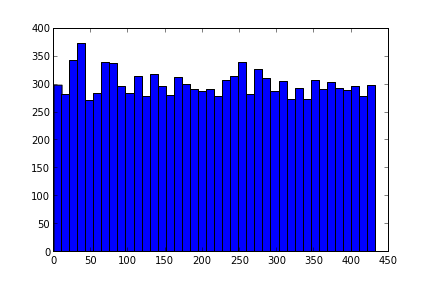
\includegraphics[height=6cm]{05_02.png}

\begin{minted}[fontsize=\footnotesize]{python}
print np.mean(data)
\end{minted}

\begin{verbatim}
213.948899167
\end{verbatim}

\begin{minted}[fontsize=\footnotesize]{python}
print np.median(data)
\end{minted}

\begin{verbatim}
214.06
\end{verbatim}

\begin{minted}[fontsize=\footnotesize]{python}
print np.std(data)
\end{minted}

\begin{verbatim}
125.118481954
\end{verbatim}

\begin{minted}[fontsize=\footnotesize]{python}
print np.mean(data)+2*np.std(data)
\end{minted}

\begin{verbatim}
464.185863074
\end{verbatim}

\begin{minted}[fontsize=\footnotesize]{python}
print np.percentile(data, 95)
\end{minted}

\begin{verbatim}
410.4115
\end{verbatim}

Goruldugu gibi uc nokta hesabi icin ortalamadan iki sapma otesini
kullanirsak, 464.18, fakat 95. yuzdeligi kullanirsak 410.41 elde
ediyoruz. Niye? Sebep ortalamanin kendisi hesaplanirken cok uc
degerlerin toplama dahil edilmis olmasi ve bu durum, ortalamanin
kendisini daha buyuk seviyeye dogru itiyor. Yuzdelik hesabi ise sadece
sayilari siralayip belli bazi elemanlari otomatik olarak uc nokta
olarak addediyor.

Box Whisker Grafikleri

Tek boyutlu bir verinin dagilimini gormek icin Box ve Whisker grafikleri
faydali araclardir; medyan (median), dagilimin genisligini ve siradisi
noktalari (outliers) acik sekilde gosterirler. Isim nereden geliyor? Box
yani kutu, dagilimin agirliginin nerede oldugunu gosterir, medyanin
sagindada ve solunda olmak uzere iki ceyregin arasindaki kisimdir, kutu
olarak resmedilir. Whiskers kedilerin biyiklarina verilen isimdir, zaten
grafikte birazcik biyik gibi duruyorlar. Bu uzantilar medyan noktasindan
her iki yana kutunun iki kati kadar uzatilir sonra verideki "ondan az olan
en buyuk" noktaya kadar geri cekilir. Tum bunlarin disinda kalan veri ise
teker teker nokta olarak grafikte basilir. Bunlar siradisi (outlier)
olduklari icin daha az olacaklari tahmin edilir.

BW grafikleri iki veriyi dagilimsal olarak karsilastirmak icin
birebirdir. Mesela Larsen and Marx adli arastirmacilar cok az veri
iceren Quintus Curtius Snodgrass veri setinin degisik oldugunu
ispatlamak icin bir suru hesap yapmislardir, bir suru matematiksel
isleme girmislerdir, fakat basit bir BW grafigi iki setin farkliligini
hemen gosterir.

BW grafikleri iki veriyi dagilimsal olarak karsilastirmak icin
birebirdir. Mesela Larsen and Marx adli arastirmacilar cok az veri
iceren Quintus Curtius Snodgrass veri setinin degisik oldugunu
ispatlamak icin bir suru hesap yapmislardir, bir suru matematiksel
isleme girmislerdir, fakat basit bir BW grafigi iki setin farkliligini
hemen gosterir.

Python uzerinde basit bir BW grafigi 

\begin{minted}[fontsize=\footnotesize]{python}
spread= rand(50) * 100
center = ones(25) * 50
flier_high = rand(10) * 100 + 100
flier_low = rand(10) * -100
data =concatenate((spread, center, flier_high, flier_low), 0)
plt.boxplot(data)
plt.savefig('05_03.png')
\end{minted}

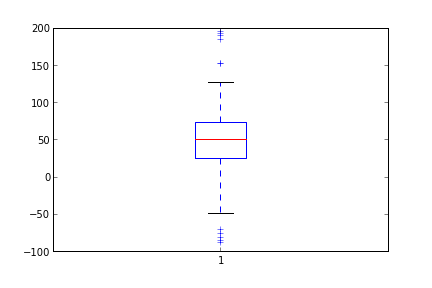
\includegraphics[height=6cm]{05_03.png}

Bir diger ornek Glass veri seti uzerinde

\begin{minted}[fontsize=\footnotesize]{python}
data = loadtxt("glass.data",delimiter=",")
head = data[data[:,10]==7]
tableware = data[data[:,10]==6]
containers = data[data[:,10]==5]

print head[:,1]

data =(containers[:,1], tableware[:,1], head[:,1])

plt.yticks([1, 2, 3], ['containers', 'tableware', 'head'])

plt.boxplot(data,0,'rs',0,0.75)
plt.savefig('05_04.png')
\end{minted}

\begin{verbatim}
[ 1.51131  1.51838  1.52315  1.52247  1.52365  1.51613  1.51602  1.51623
  1.51719  1.51683  1.51545  1.51556  1.51727  1.51531  1.51609  1.51508
  1.51653  1.51514  1.51658  1.51617  1.51732  1.51645  1.51831  1.5164
  1.51623  1.51685  1.52065  1.51651  1.51711]
\end{verbatim}

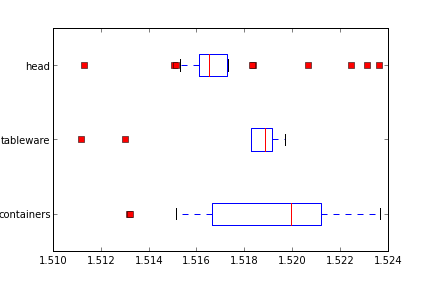
\includegraphics[height=6cm]{05_04.png}

Guven Araligi (Confidence Intervals)

Bir guven araligi tanimlamanin Bayes usulu bu hesabi bir dagilimi baz
alarak yapmak. Eger sonuc olarak bir tekil sayi degil, bir dagilim elde
edersek bu dagilim uzerinde guvenlik hesaplarini yapmak cok kolay hale
gelir. Mesela sonuc (sonsal dagilim) bir Gaussian dagilim ise, bu dagilimin
yuzde 95 agirliginin nerede oldugu, ve nasil hesaplandigi bellidir.

Bayes Teorisi

$$ P(A|B)  = \frac{ P(B|A)P(A)}{P(B)} $$

Veri analizi baglaminda diyelim ki deneyler yaparak tahmini olarak
hesaplamak (estimate) istedigimiz bir parametre var, bu bir protonun
kutlesi ya da bir ameliyat sonrasi hayatta kalma orani olabilir. Bu
durumlarda iki ayri "olaydan" bahsetmemiz gerekir, B olayi spesifik bazi
olcumlerin elde edilmesi "olayidir", mesela olcum uc sayidan olusuyorsa,
biz bir olcumde spesifik olarak $\{0.2,4,5.4\}$ degerlerini elde
etmisiz. Ikinci olay bilmedigimiz parametrenin belli bir degere sahip
olmasi olacak. O zaman Bayes Teorisinin su sekilde tekrar yazabiliriz, 

$$ P(parametre | veri ) \propto P(data | parametre)P(parametre) $$

$\propto$ isareti orantili olmak (proportional to) anlamina geliyor. Boleni
attik cunku o bir sabit (tamamen veriye bagli, tahmini hesaplamak
istedigimiz parametreye bagli degil). Tabii bu durumda sol ve sag taraf
birbirine esit olmaz, o yuzden esitlik yerine orantili olmak isaretini
kullandik. Bu cercevede "belli bir numerik sabit cercevesinde birbirine
esit (equal within a numeric constant)" gibi cumleler de gorulebilir. 

Ornek

Diyelim ki bir bozuk para ile 10 kere yazi-tura attik, ve sonuc altta

T H H H H T T H H H

Bu veriye bakarak paranin hileli olup olmadigini anlamaya
calisacagiz. Bayes ifadesini bu veriye gore yazalim,

$$ P(p | \{ \textrm{T H H H H T T H H H} \} \propto 
P(\{ \textrm{T H H H H T T H H H} | p) P(p) \}
$$

$P(p)$ ifadesi ne anlama gelir? Aslinda bu ifadeyi $P([Dagilim] = p)$
olarak gormek daha iyi, artik $p$ parametresini bir dagilimdan gelen bir
tekil deger olarak gordugumuze gore, o dagilimin belli bir $p$'ye esit
oldugu zamani modelliyoruz burada. Her halukarda $P(p)$ dagilimini, yani
onsel (prior) olasiligi bilmiyoruz, hesaptan once her degerin mumkun
oldugunu biliyoruz, o zaman bu onsel dagilimi duz (flat) olarak aliriz,
yani $P(p) = 1$. 

$P(\{\textrm{T H H H H T T H H H} | p)$ ifadesi goz korkutucu olabilir, ama
buradaki her ogenin bagimsiz ozdesce dagilmis (independent identically
distributed) oldugunu gorursek, ama bu ifadeyi ayri ayri
$P(\{\textrm{T}|p)$ ve $P(\{\textrm{H}|p)$ carpimlari olarak gorebiliriz. $P(\{\textrm{T}|p) = p$ ve 
$P(\{\textrm{H}|p)=1-p$ oldugunu biliyoruz. O zaman 

$$ P(p | \{ \textrm{7 Tura, 3 Yazi} \} \propto
p^7(1-p)^3
$$

Grafiklersek, 

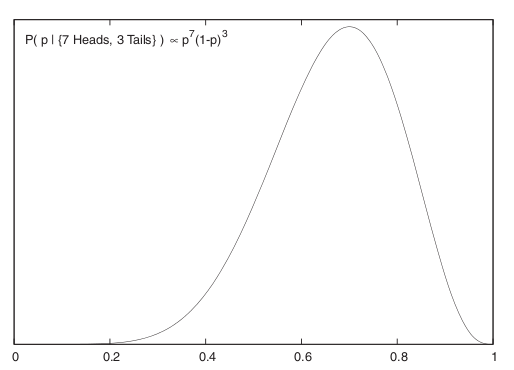
\includegraphics[height=6cm]{05_01.png}

Boylece $p$ icin bir sonsal (posterior) dagilim elde ettik. Artik bu
dagilimin yuzde 95 agirliginin nerede oldugunu rahatca gorebiliriz /
hesaplayabiliriz. Dagilimin tepe noktasinin $p=0.7$ civarinda oldugu
goruluyor. Bir dagilimla daha fazlasini yapmak ta mumkun, mesela bu
fonksiyonu $p$'ye bagli baska bir fonksiyona karsi entegre etmek mumkun,
mesela beklentiyi bu sekilde hesaplayabiliriz. 

Onsel dagilimin her noktaya esit agirlik veren birornek (uniform) secilmis
olmasi, yani problemi cozmeye sifir bilgiden baslamis olmamiz, yontemin bir
zayifligi olarak gorulmemeli. Yontemin kuvveti elimizdeki bilgiyle baslayip
onu net bir sekilde veri ve olurluk uzerinden sonsal tek dagilima
goturebilmesi. Baslangic ve sonuc arasindaki baglanti gayet net. Fazlasi da
var; ilgilendigimiz alani (domain) ogrendikce, basta hic bilmedigimiz onsel
dagilimi daha net, bilgili bir sekilde secebiliriz ve bu sonsal dagilimi da
daha olmasi gereken modele daha yaklastirabilir. 

\end{document}
